\subsection{Developers Using AdaptUI}
\label{sec:developers}

Before introducing the results obtained from working with final users (as 
consumers of adapted user interfaces), an experiment with developers has been 
performed. This experiment aims to evaluate the provided \acp{api}, and also to 
compare the differences between performing a configuration of the user interface 
in Android with and without AdaptUI. Thus, developers with experience in both 
Android development and semantics are involved.

As AdaptUI provides an \ac{api} conceptually divided in two (see 
Section~\ref{sec:application_layer}), this experiment has been fragmented 
accordingly. The experiment, consisting in 6 steps and with a 20 minutes duration,
has been carried out as follows:

\begin{enumerate}
  \item First, the developer is introduced to the AdaptUI framework through a brief
  explanation of AdaptUI's goals, virtues and boundaries. Both \acp{api} are 
  described and explained to them, and the \acp{api} descriptions are given in a 
  printed version, as they appear in Table~\ref{tbl:api_adaptation} and
  Table~\ref{tbl:api_knowledge}.
  
  \item Secondly, a Java project built with the Eclipse \acs{ide} is presented. 
  This project uses the AdaptUI framework as an imported library. The main class 
  of this Java application instantiates AdaptUI and initializes the environment. 
  Besides, several \textit{TODO} tasks with the corresponding instructions are 
  given for the developer to complete. This class is summarized through
  Listing~\ref{lst:default_knowledge_experiment}. These tasks include:
  \begin{itemize}
    \item The creation of a new class.
    \item The creation of a new instance of the previously created class.
    \item Adding a new datatype property with the corresponding value to the
    new instance.
    \item Adding a new object property to the new instance, involving several
    classes\footnote{As the developer might not know how the AdaptUIOnt ontology
    is structured, a brief explanation is given using Protégé.}.
    \item The creation of a new rule, involving at least three classes (including
    the created class), and the previous mentioned datatype and object properties.
  \end{itemize}

  \inputminted[linenos=true, fontsize=\footnotesize, frame=lines]{java}{5_experiments_and_results/default_knowledge_experiment.java}
  \captionof{listing}{The default main class with the corresponding tasks to
  be accomplished by the developer.\label{lst:default_knowledge_experiment}}

  \item Once the corresponding knowledge modifications are made, the resulting
  ontology is stored. Developers are requested to check the changes in the ontology
  using Protégé. Figure~\ref{fig:protege} shows an example of a modified ontology 
  by a participating developer. Hence, the developer is allowed to check if the 
  changes made in the Java main class using the AdaptUI framework have been 
  correctly represented in the ontology. If any errors are found, the process is 
  revised.

  \begin{figure}
  \centering
  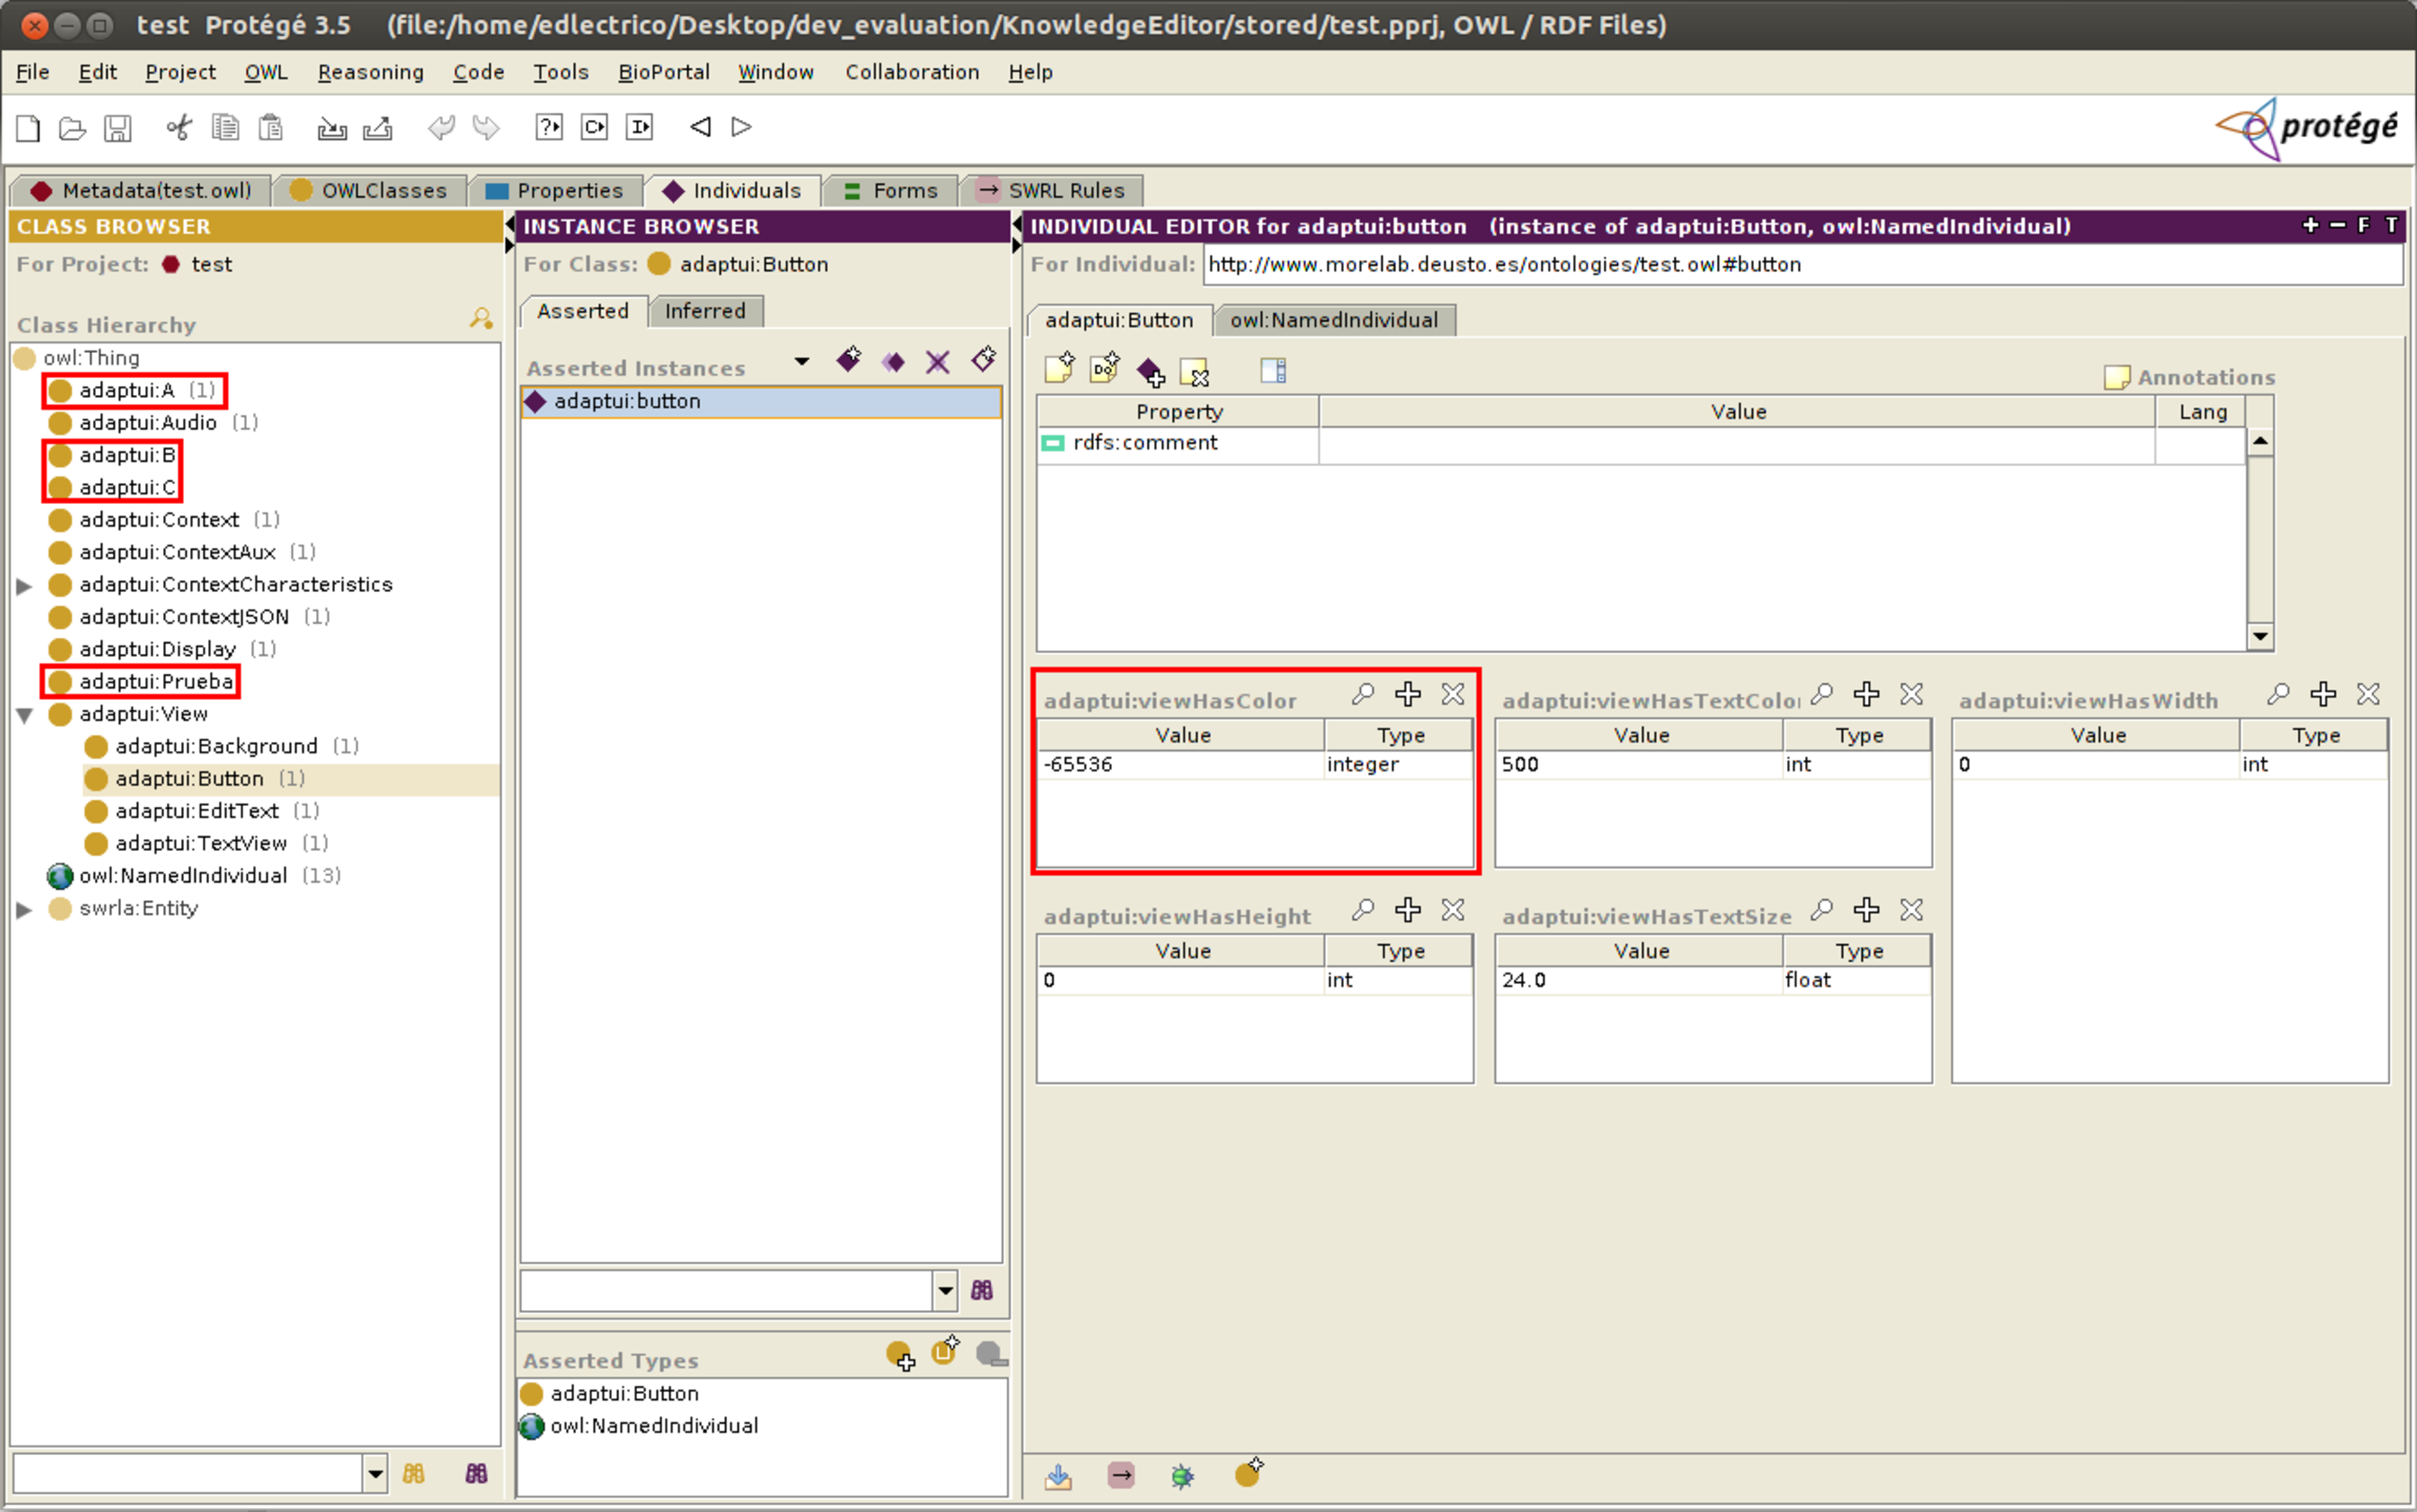
\includegraphics[width=0.85\textwidth]{protege.pdf}
  \caption{A test ontology modified by one of the participating developers. 
  The modifications are highlighted in red. Several classes have been added. 
  Also the \textit{viewBackgroundColor} for the \textit{Button} only instance 
  has been modified.}
  \label{fig:protege}
  \end{figure}
  
  \item After the modification of the ontology, the AdaptUIDemo Android project 
  is presented to the developer. This project's main activity shows a text view, 
  an edit text and a button. The goal of this part of the experiment is to evaluate
  how the developer uses the adaptation \ac{api} to dynamically modify these views.
  The changes performed in the ontology in the previous steps are taken into account. 
  In order to make this application to use the new modified version of the ontology, 
  an \acs{adb} command is needed. This command pushes the required file from the 
  current computer disk to the desired Android folder. Listing~\ref{lst:adb_push} 
  shows how the command \acs{adb} push command works.
  
  \inputminted[linenos=true, fontsize=\footnotesize, frame=lines]{java}{5_experiments_and_results/adb_push.java}
  \captionof{listing}{The \ac{adb} push command. The first parameter specifies  
  the location of the file to be sent to the device. The second parameter points
  at the absolute location in the device. \label{lst:adb_push}}
  
  \item Next, once the developer checks that the adaptation to the views shown
  in the demo application matches the modifications performed with the knowledge 
  \ac{api}, the developer is asked to use the adaptation \ac{api} through an
  Android project. Similar to the first case, the developer is asked to complete
  several tasks (see Listing~\ref{lst:default_adaptation_experiment}).

  \inputminted[linenos=true, fontsize=\footnotesize, frame=lines]{java}{5_experiments_and_results/default_adaptation_experiment.java}
  \captionof{listing}{The default Android version with the corresponding tasks to
  be completed by the developer. These tasks include adapting the background and
  text colour of a button, its size and the background colour of the whole activity\label{lst:default_adaptation_experiment}}
  
  \item Finally, the developer uses the Capabilities Collector to adapt several
  views as a user. As the last task of the Capabilities Collector is to store the
  required values in the ontology through the Semantic Modeller, the developer 
  is able to check these changes again in the AdaptUIDemo application.
  
\end{enumerate}



% The following sections aim to give more details about the experiments defined
% above.
% 
% \subsubsection{Using the knowledge editor \ac{api}}
% \label{sec:knowledge_editor_api}
% 
% The knowledge editor \ac{api} provides a set of methods to modify the knowledge
% stored in the ontology. Imported as a library from a Java project, this \ac{api}
% allows to add and remove classes, individuals, object and datatype properties,
% and rules. In this experiment developers are asked to modify the ontology by
% adding new concepts to be used by the adaptation \ac{api}.
% Listing~\ref{lst:adaptui_add_knowledge} shows an example of how developers can
% modify the knowledge stored in the ontology.
% 
% \inputminted[linenos=true, fontsize=\footnotesize, frame=lines]{java}{5_experiments_and_results/adaptui_add_knowledge.java}
% \captionof{listing}{Modifying the knowledge represented in the ontology through the knowledge \ac{api}.\label{lst:adaptui_add_knowledge}}
% 
% \subsubsection{Using adaptation \ac{api}}
% \label{sec:adaptation_api_experiment}
% 
% As mentioned in Section~\ref{sec:adaptation_api}, the adaptation \ac{api} provides 
% a set of methods whose purpose is to facilitate the adaptation process for 
% developers. The purpose of this part of the experiment is to check developer's 
% feedback when dealing with the AdaptUI framework by collecting their opinions.
% To do so, the experiment presents an Android application developed with the 
% Eclipse\footnote{https://eclipse.org/} \ac{ide}. It includes a layout configuration 
% \ac{xml} file with the corresponding declaration of several user interface views
% (see Listing~\ref{lst:default_layout}), and also an \textit{onCreate} main method, 
% shown in Listing~\ref{lst:default_oncreate} (the default aspect of the application
% is illustrated through Figure~\ref{fig:default_layout}). The developers 
% participating in this experiment are guided through a brief explanation of the 
% available adaptation \ac{api} methods. Once they are aware of the possibilities 
% the framework provides, they are asked to modify the aspect of the listed views.
% 
% \inputminted[linenos=true, fontsize=\footnotesize, frame=lines]{xml}{5_experiments_and_results/default_layout.xml}
% \captionof{listing}{The default layout defining a grid layout, a text view,
% a button and an edit text.\label{lst:default_layout}}
% 
% \inputminted[linenos=true, fontsize=\footnotesize, frame=lines]{java}{5_experiments_and_results/default_oncreate.java}
% \captionof{listing}{The default \textit{onCreate} method.\label{lst:default_oncreate}}
% 
% \begin{figure}
% \centering
% 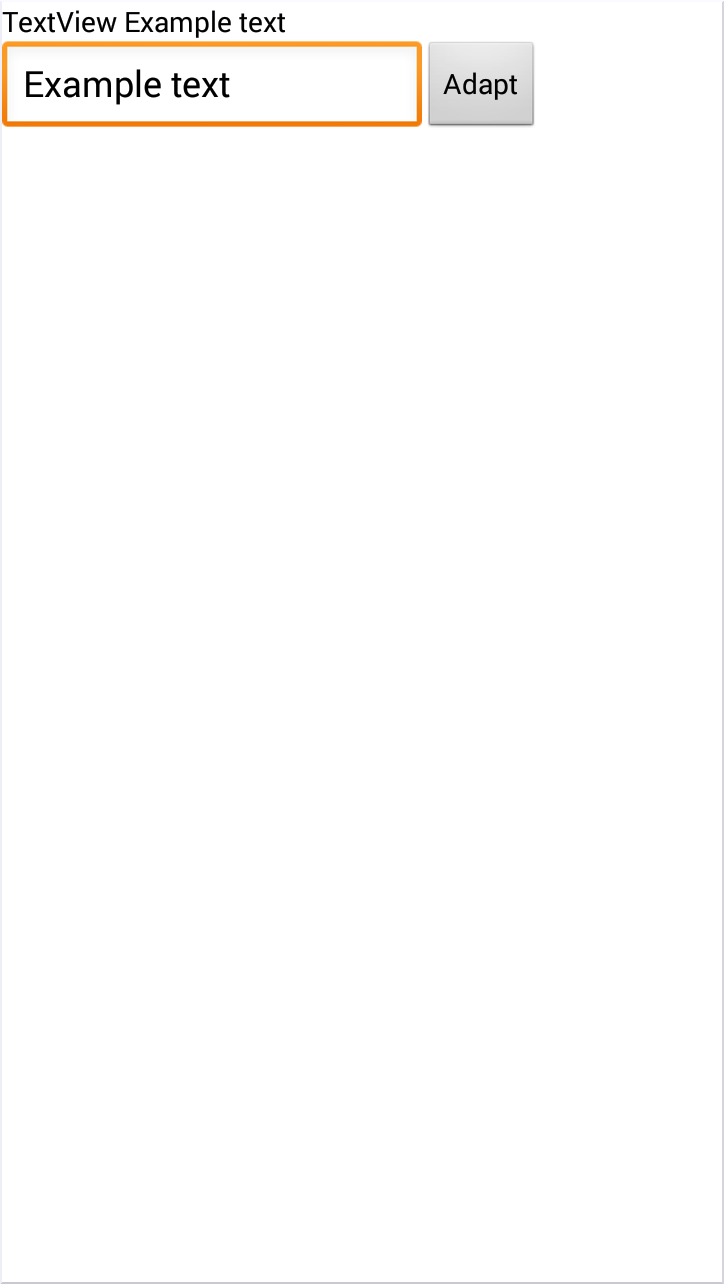
\includegraphics[width=0.25\textwidth]{default_layout.png}
% \caption{The corresponding user interface considering the layout specified in
% Listing~\ref{lst:default_layout}.}
% \label{fig:default_layout}
% \end{figure}
% 
% Obviously, in order to adapt the application, developers need a copy of the
% AdaptUIOnt ontology, in which the corresponding values for the adaptation are
% semantically represented. Hence, developers are asked to install the Capabilities 
% Collector in their Android devices. Thus, they can add new knowledge to the ontology.
% 
% Listing~\ref{lst:default_oncreate} shows the presented \textit{onCreate} method, 
% which defines the views listed in Listing~\ref{lst:default_layout}. Using AdaptUI 
% developers reach the \textit{onCreate} shown in Listing~\ref{lst:adaptui_oncreate},
% which includes the corresponding calls to the provided adaptation \ac{api}.
% 
% \inputminted[linenos=true, fontsize=\footnotesize, frame=lines]{java}{5_experiments_and_results/adaptui_oncreate.java}
% \captionof{listing}{The AdaptUI \textit{onCreate} method.\label{lst:adaptui_oncreate}}
% 
% Thus, the resulting adapted user interface is illustrated by Figure~\ref{fig:adapted_layout}.
% While Figure~\ref{fig:default_layout} shows a default disposition and configuration
% of the user interface items described in Listing~\ref{lst:default_layout}, in this
% case they have been adapted according to Listing~\ref{lst:adaptui_oncreate}.
% 
% \begin{figure}
% \centering
% 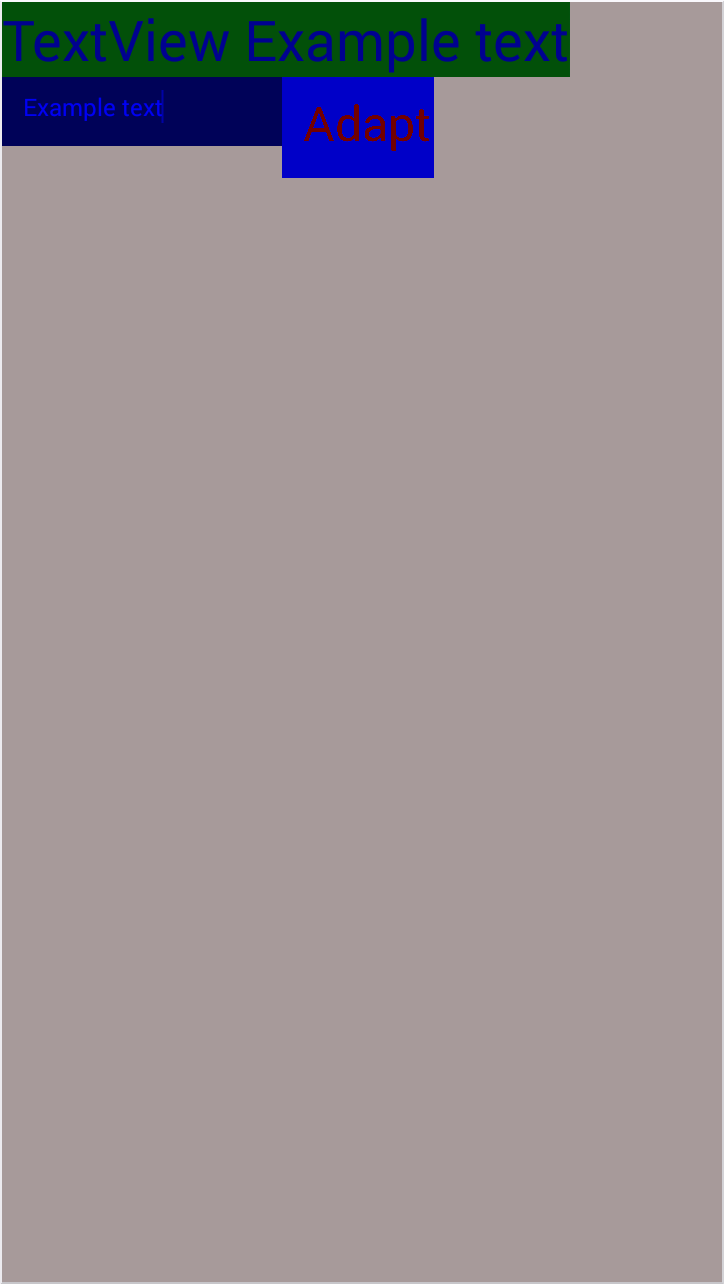
\includegraphics[width=0.25\textwidth]{adapted_layout.png}
% \caption{The corresponding user interface considering the layout specified in
% Listing~\ref{lst:adaptui_oncreate}.}
% \label{fig:adapted_layout}
% \end{figure}


\subsubsection{Results and Conclusions}
\label{sec:api_results}

The resulting experiences with the provided \acp{api} have been collected through
a simple questionnaire. It is a very straightforward questionnaire, not based on
any standard. Its purpose is to find out if the participating developers miss 
any possible feature and to gather their feedback about AdaptUI. The 
questionnaire is formed by the following questions:

\begin{enumerate}
 \item \#Q1: How useful do you find the AdaptUI framework for developing adaptive 
 user interfaces?\footnote{This question requires the user to select a value from
 a 1 to 5 scale, 1 meaning \textit{not much} and 5 meaning \textit{very much}.}
 \item \#Q2: Do you miss any additional functionality?
 \item \#Q3: If so, please specify the functionality you would add to the 
 framework/\ac{api}.
 \item \#Q4: Would you improve any \ac{api} feature?
 \item \#Q5: If so, which one and how?
 \item \#Q6: Would you make AdaptUI part of your future applications (if you 
 plan to use adaptive interfaces)?
 \item \#Q7: Comments.
\end{enumerate}

The developers' responses are gathered in Table~\ref{tbl:developers_responses}
and Table~\ref{tbl:developers_responses_2}. The results show that the participating 
developers have found the AdaptUI \ac{api} very useful. The comments, as expected, 
reveal that they would find it more useful if a \acs{oop} paradigm is followed. 
In the current version the definition and modification of the knowledge and of 
the adaptation is more declarative. These considerations are gathered in 
Section~\ref{sec:future_work}.

\begin{table}
  \caption{Developers' responses to the questionnaire. As responses for questions 
  \#Q3, \#Q5 and \#Q7 might be too long, their details are given in 
  Table~\ref{tbl:developers_responses_2}. If a response for any of these questions
  is given by the developer an asterisk symbol(*) is shown in the corresponding
  cell.}
 \label{tbl:developers_responses}
\footnotesize
\centering
 \begin{tabular}{l l l l l l l l}
  \hline 
  \textbf{\#Developer} 	& \textbf{\#Q1} & \textbf{\#Q2} & \textbf{\#Q3} & \textbf{\#Q4} & \textbf{\#Q5} & \textbf{\#Q6} & \textbf{\#Q7} \\
  \hline
  \#1			& 4		& Yes		& * 		& Yes	 	& - 		& Yes 		& - \\
  \#2			& 5		& No		& - 		& Yes		& *		& Yes		& - \\
  \#3			& 5		& No		& - 		& No		& -		& Yes		& - \\
  \#4			& 4		& No		& - 		& Yes		& *		& Yes		& - \\
  \#5			& 4		& No		& - 		& Yes		& *		& Yes		& * \\
  \hline
\end{tabular}
\end{table}

\begin{table}
  \caption{Developers' responses to questions \#Q3, \#Q5 and \#Q7.}
 \label{tbl:developers_responses_2}
\footnotesize
\centering
 \begin{tabular}{l l l l l l l l}
  \hline 
  \textbf{\#Developer} 	& \textbf{\#Q3} 		& \textbf{\#Q5} 	& \textbf{\#Q7}	\\
  \hline
  \#1			& To be able to define more	& -			& -		\\
			& than one configuration for 	& 			& 		\\
			& the same view.		& 			& 		\\
  \#2			& -				& \acs{oop} paradigm.	& -		\\
  \#3			& -				& -			& -		\\
  \#4			& - 				& Pass the object to	& \acs{oop} paradigm.	\\
			&				& the adaptation method & 		\\
			&				& as parameter.		& 		\\
  \#5			& -				& Pass the object to	& This is my first \\
			& 				& the adaptation method	& experience with  \\
			& 				& as parameter.		& ontologies, and I've \\
			&				&			& found it satisfactory. \\
  \hline
\end{tabular}
\end{table}


